\documentclass[conference]{IEEEtran}

\usepackage{cite}
\usepackage{booktabs}
\usepackage{graphicx}
\usepackage{xcolor}
\usepackage{url}
\usepackage{placeins}

% Let tall two-column figures sit at the top of a page together with text (default limit is 0.7 of the page).
\renewcommand{\dbltopfraction}{0.9}
\renewcommand{\dblfloatpagefraction}{0.7}

% Visible marker for anything the author still has to fill in or verify.
\newcommand{\todo}[1]{\textcolor{red}{[TODO: #1]}}

\begin{document}

\title{Observability and Evaluation Tools for AI Agents: Tool Selection, Built-in Metrics and a Metric Taxonomy}  % TODO: confirm title; IEEE allows no subtitle

\author{\IEEEauthorblockN{1\textsuperscript{st} \todo{Given Name Surname}}
\IEEEauthorblockA{\textit{\todo{dept. name of organization}} \\
\textit{\todo{name of organization}}\\
\todo{City, Country} \\
\todo{email address or ORCID}}}

\maketitle

\begin{abstract}
\todo{Rewrite once the structure is settled.}
AI agents run many model calls and tool calls per task, and a growing number of tools claim to observe and evaluate them. We ask which tools are most widely named in public sources and which agent-execution metrics they provide out of the box.
Following an adapted multivocal search over GitHub, the web and the OpenTelemetry standard, we selected 13 tools and collected 241 built-in metrics from their official documentation, each with a source URL, a verbatim quote and an access date.
Merging equivalent metrics yields a taxonomy of 46 unique metrics in 13 categories: 19 observability metrics (whose values are captured from a run) and 27 evaluation metrics (whose values are judgements of agent behaviour or output).
A worked example on a retrieval-augmented chatbot, traced with Langfuse and scored with Arize Phoenix and DeepEval, shows 30 of the 46 metrics reported by these three tools in a single run, and shows that a failure the application does not flag as an error is missed by the tracer's error metrics but caught by evaluators.
\end{abstract}

\begin{IEEEkeywords}
AI agents, observability, evaluation, LLM, metrics, taxonomy \todo{confirm keywords}
\end{IEEEkeywords}

\section{Introduction}
\todo{Motivation: agents are non-deterministic, multi-step and tool-using, so a final answer alone says little about how a run went. Say why metrics need to be chosen deliberately, and why the vocabulary differs between tools.}

This paper makes three contributions:
\begin{enumerate}
  \item A selection of 13 observability and evaluation tools for AI agents, made with written rules from logged GitHub and Google queries (Section~\ref{sec:method}).
  \item A catalogue of 241 built-in metrics from those tools, each tied to documentation evidence, and a taxonomy of 46 unique metrics (Section~\ref{sec:results}).
  \item A motivating example that shows, on one real application, which of these metrics three of the tools report and where they disagree (Section~\ref{sec:example}).
\end{enumerate}
Section~\ref{sec:related} defines the basic terms, shows how the tools build on common telemetry standards, reviews related work and ends with the motivating example. Section~\ref{sec:method} covers the method, Section~\ref{sec:results} the results, and Sections~\ref{sec:discussion}--\ref{sec:limits} the discussion and limitations.
\todo{Research questions, if the venue expects them (for example: RQ1 which tools; RQ2 which built-in metrics; RQ3 how do metrics overlap across tools).}

\section{Background, Related Work and Example}\label{sec:related}
This section fixes the vocabulary used in the rest of the paper, explains how the tools relate to the telemetry standards they build on, positions the paper against earlier work, and then shows on one real application what a tracing tool and two evaluators report.

\subsection{Basic terms}\label{sec:terms}
\emph{Observability} is the ability to understand what a system did from the data it emits; for an LLM agent, this is a record of every model call and tool call made while solving a task. \emph{Evaluation} judges whether what the agent did, and what it answered, was good. The first is recorded; the second needs a judge: a rule, a model or a person. The tools studied here offer one or both.

To say what is recorded, we need a unit. A \emph{run} is one execution of the agent, from an input (a user question or a task) to its final output. The data recorded for one run is a \emph{trace}. A trace is made of \emph{spans}. A span is one timed operation with a start, an end, a parent and attributes (model name, token counts, tool name, input, output), so spans nest. A \emph{step} is one action of the agent, a model call or a tool call, and usually corresponds to one span; spans also record other work, such as a retrieval. A \emph{session} groups the runs of one conversation. Tools use different words for the same ideas (Table~\ref{tab:terms}); in particular, LangSmith calls a span a ``run''. In this paper ``run'' always means the whole execution.

\begin{table}[t]
\centering
\scriptsize
\setlength{\tabcolsep}{2pt}
\begin{tabular}{@{}lccccc@{}}
\toprule
Term here & OTel & Phoenix & LangSmith & Langfuse & Weave \\
\midrule
Run (whole) & trace & trace & trace & trace & trace \\
Step (one op.) & span & span & run & observation & call \\
\bottomrule
\end{tabular}
\caption{The same ideas under different names, from each tool's documentation.}
\label{tab:terms}
\end{table}

With the unit fixed, we can say what is computed from it. A \emph{metric} is a named, defined quantity. It states what is measured (a span, a run or a set of runs), the unit or scale, and how results are combined, so that it can be computed again and compared. ``LLM call latency'' is a metric. A \emph{measurement} is a number obtained by applying such a metric to what was recorded: this model call took 3.1~s, or the median over twelve runs was 3.0~s. A \emph{score} is the number an evaluator assigns to an output or a behaviour, for example a faithfulness of 0.9 given by an LLM judge. We call a metric an \emph{observability metric} when it is computed from measurements captured during the run (tokens, cost, latency, counts, errors) and an \emph{evaluation metric} when it is a score from a judgement. The difference matters in use: a measurement is read from the trace, while a score depends on the judge (its prompt, its model or its reviewer) and can change when the judge changes.
Each tool's own metric is a \emph{tool-specific metric}, with its own procedure; a \emph{unique metric} groups tool-specific metrics that measure the same property (Section~\ref{sec:taxonomy}), so two tools can report different measurements for one unique metric.

\subsection{Standards underneath the tools}\label{sec:stack}
Most of the tools studied sit on a shared telemetry layer, which shapes what they can report. The layer has three levels. At the bottom, \emph{conventions} fix the names and meaning of span attributes and metrics: the OpenTelemetry GenAI semantic conventions~\cite{otelgenai} (attributes named \texttt{gen\_ai.*}) and OpenInference~\cite{tool_openinference} (attributes named \texttt{llm.*}), which is itself built on OpenTelemetry. In the middle, \emph{instrumentation libraries} wrap an LLM or an agent framework and emit spans that follow a convention. OpenLLMetry~\cite{tool_openllmetry} describes itself as a set of extensions built on top of OpenTelemetry, and states that its conventions are now part of OpenTelemetry. At the top, \emph{platforms} store and display the spans and compute metrics from them, and \emph{frameworks} run evaluators.

The documentation of the platforms shows how tightly they are tied to this layer (Table~\ref{tab:tools}, last column). Phoenix is built on OpenTelemetry and powered by OpenInference instrumentation; Langfuse is built on OpenTelemetry and reads token counts from both \texttt{gen\_ai.usage.*} and \texttt{llm.token\_count.*} attributes; Galileo's OTLP endpoint follows both conventions; LangSmith, Opik and Braintrust accept OpenTelemetry traces; promptfoo can trace the providers it evaluates with OpenTelemetry. For Weave we only found that its calls are modelled like OpenTelemetry spans, and in the pages read Helicone and DeepEval show no OpenTelemetry link.

Two consequences follow. First, the observability metrics are largely the same across tools because they are read from the same attributes: Phoenix derives cost from the OpenInference token-count attributes, and the OpenTelemetry conventions define the same quantities as metrics (duration of an agent invocation, counts of tool calls and model calls, token usage). Agreement between two tools on tokens, latency or counts is therefore weaker evidence than agreement between independent designs. Second, in the pages we read, the conventions give an attribute for the score an evaluator produced but no list of evaluation metrics. Faithfulness or task completion is defined by each tool, and this is where the vocabularies differ most.

\subsection{Related work}\label{sec:prior}
Two earlier studies are closest to ours: one compares tools, the other organises evaluation approaches.

The first is Dong et al.~\cite{dong2024agentops}, who built a taxonomy of AgentOps from a mapping study of 17 tools found through GitHub and Google search in November 2024, the same two sources we use. They compare the tools on seven feature groups (customisation, prompt management, evaluation, feedback, monitoring, tracing, guardrails), each marked yes or no, and their taxonomy lists the artifacts that should be traced over an agent's life cycle. We go one level down: instead of asking whether a tool has a feature, we record which built-in metrics it documents, each with a quotation from the documentation and an access date, and we group what the tools compute rather than what should be traced. Our tools are also chosen by written rules rather than a keyword search (Section~\ref{sec:method}), and the set is current (2026); only five of our 13 tools (Langfuse, LangSmith, Phoenix, Helicone, OpenLLMetry) are among their 17.

Yehudai et al.~\cite{yehudai2025survey} approach the problem from the evaluation side. They compare eight evaluation frameworks, four of which are also in our set (LangSmith, Langfuse, Arize Phoenix, Galileo), and organise evaluation by granularity: final response, stepwise (tool selection, parameters, progress toward a goal) and trajectory (alignment with a reference path), with monitoring (task completion, latency, throughput) as a separate capability. Our metrics fit this view: answer quality, grounding, safety and conversation metrics correspond to final-response evaluation; tool-use and goal-progress metrics to stepwise evaluation; plan and trajectory metrics to trajectory evaluation; and token, cost, latency and error metrics to monitoring (Section~\ref{sec:results}). Where we go further is detail. Their frameworks are rated yes or no per capability, whereas we list each metric and separate observability from evaluation metrics. Their monitoring column is a single item, which we split into separate metrics such as cached and reasoning tokens or time to first token. They also present cost and safety as open directions for evaluation, while in the pages we read several of the 13 tools already document built-in metrics for both. \todo{Check this comparison against the PDF of Yehudai et al. and the final taxonomy before submission.}

The remaining work is further from ours. Wang et al.~\cite{wang2025agentops} tabulate monitoring tools by whether they offer logs, traces, and system, cost, RAG and performance metrics, and Mohammadi et al.~\cite{mohammadi2025evaluation} organise agent evaluation by objective and process, naming tools only in passing. Solomon et al.~\cite{solomon2025lumimas} list in an appendix the kinds of data each tool collects (tokens, latency, cost, errors), but at the level of metric families. Souza and Machado~\cite{souza2026architecture} propose to map agent components and behaviours to metrics from LangSmith, DeepEval and Opik, but the mapping is not yet published. Finally, the multivocal method has been applied to ML monitoring~\cite{naveed2025monitoring}, though not to LLM agents.

Taken together, we found no work that extracts the built-in metrics of each tool from its documentation with a quotation and access date, or that groups them into one taxonomy. We looked for such work with eight queries on arXiv and ACM, IEEE and ACL sources on 2026-10-30; the search was not exhaustive (Section~\ref{sec:limits}).

\subsection{Motivating example}\label{sec:example}
This subsection shows, on one real application, what observability and evaluation tools report about runs of an LLM agent. It illustrates what such tools produce in practice; it does not evaluate them.

\subsubsection{Setup}
The application is the course chatbot from the DeepLearning.AI course on Claude Code \todo{full citation and URL}: a single LLM with two tools, \texttt{search\_\allowbreak course\_\allowbreak content} and \texttt{get\_\allowbreak course\_\allowbreak outline}, answering questions over four course transcripts. We ran it on \texttt{gpt-5-mini} and traced it with Langfuse~\cite{tool_langfuse}. Twelve scripted questions in nine sessions covered factual questions answerable from the transcripts, one question the transcripts cannot answer, a general-knowledge question, and a four-turn conversation. The expected answers were taken from the transcripts and written before the run. The recorded turns were then scored offline with the built-in evaluators of Arize Phoenix~\cite{tool_arize_phoenix} and DeepEval~\cite{tool_deepeval}, using \texttt{gpt-5-mini} as judge. The application and the questions are described in the accompanying repository (\texttt{example\_rag}). As an illustration, Fig.~\ref{fig:graph} shows the graph Langfuse draws for one of the twelve runs, a question about deploying MCP servers on Kubernetes that the transcripts cannot answer: the model made three calls and two searches.

\begin{figure}[!t]
\centering
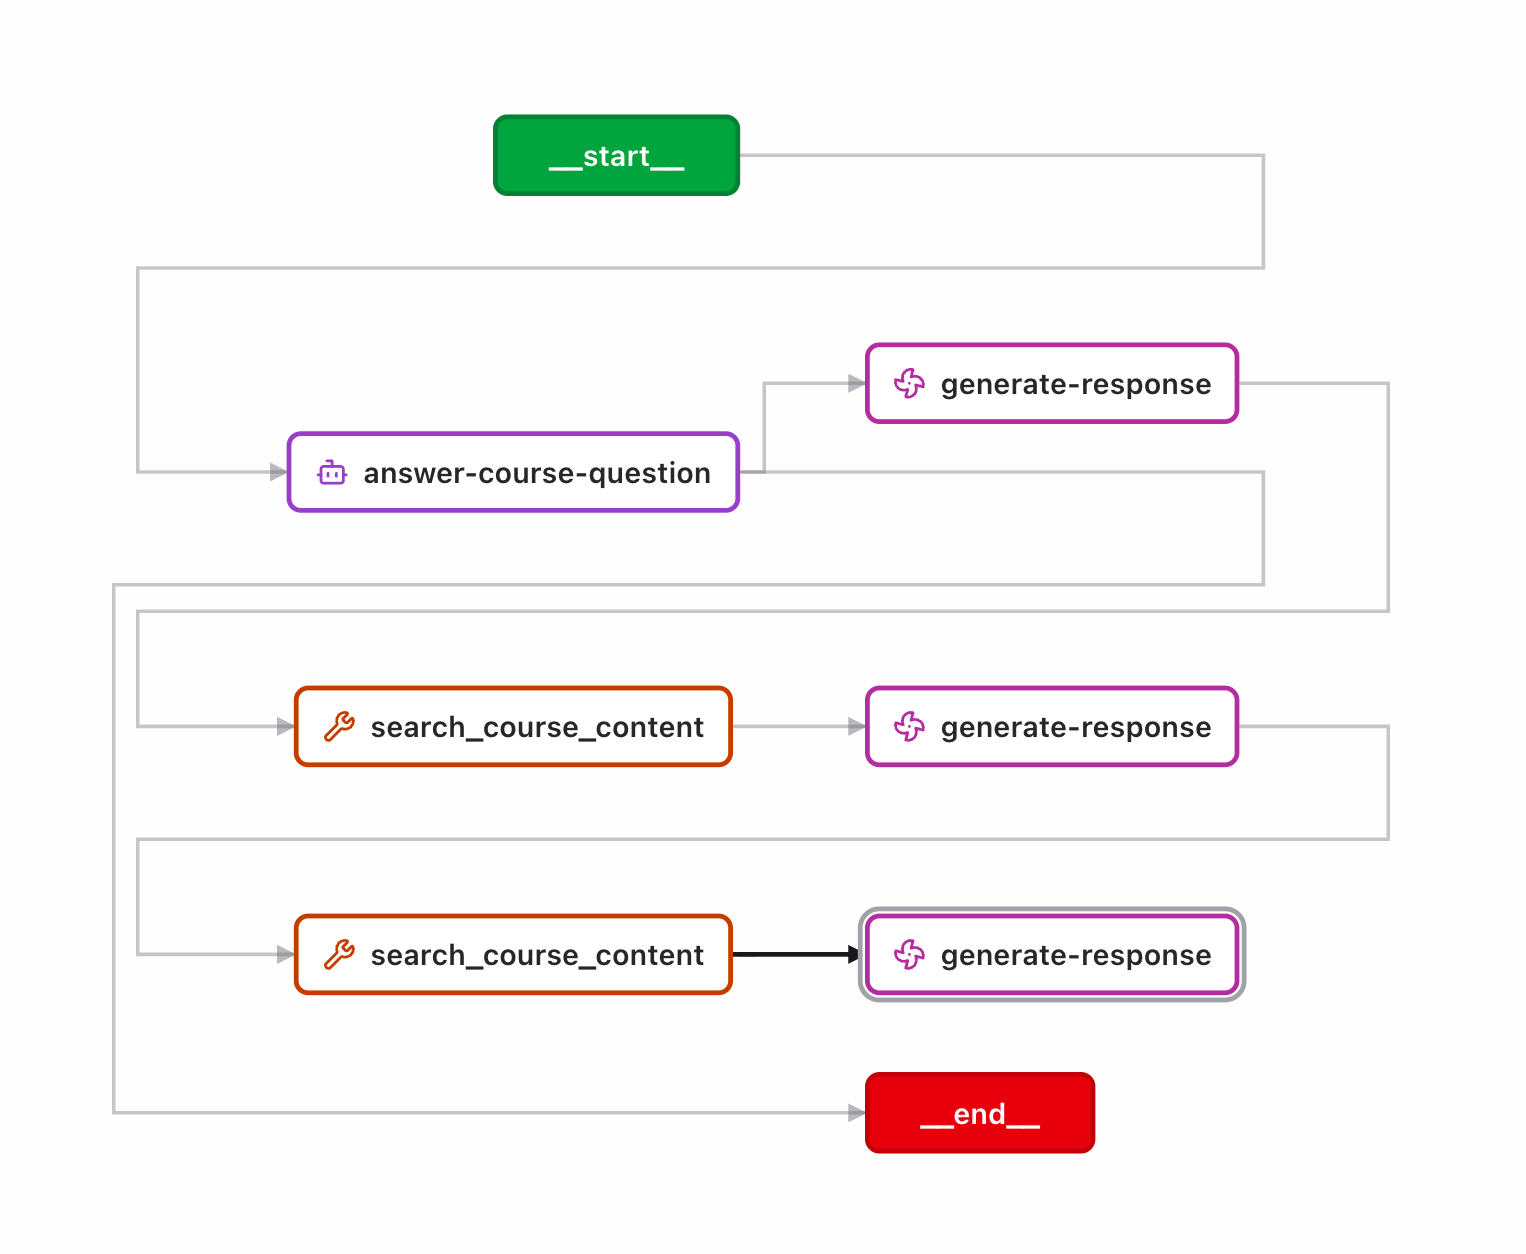
\includegraphics[width=\columnwidth]{figures/langfuse_graph_s7.png}
\caption{Langfuse agent graph for the question about deploying MCP servers on Kubernetes: three model calls (\texttt{generate-response}) and two searches. The first search returned ``No course found matching `MCP'\,''; the second returned course content.}
\label{fig:graph}
\end{figure}

\subsubsection{What the tools reported}
Over the twelve runs, Langfuse reported 12 traces and 44 observations, 22 model calls and 10 tool calls; 19,684 input, 2,598 output and 5,632 reasoning tokens (Langfuse counts reasoning tokens apart from output tokens, so its total of 27,914 is the sum of the three); a cost of \$0.0214 split by token type; and latency per run, per model call and per tool call. It reported no first-token time because the application does not stream. Phoenix evals and DeepEval scored the twelve runs on tool selection, tool argument validity, tool call correctness, tool response handling, task completion, answer relevance, conciseness, faithfulness to the retrieved context, toxicity, bias, sensitive-data leakage, refusal, knowledge retention and user frustration. Tokens, cost and latency are Langfuse's own values; the counts of calls and observations were computed from its observation records. Fig.~\ref{fig:example} lists the 30 metrics the tools reported (rows) and what each tool reported for each: measurements for the metrics recorded by the tracer, scores for those computed by the evaluators.

\begin{figure*}[!t]
\centering
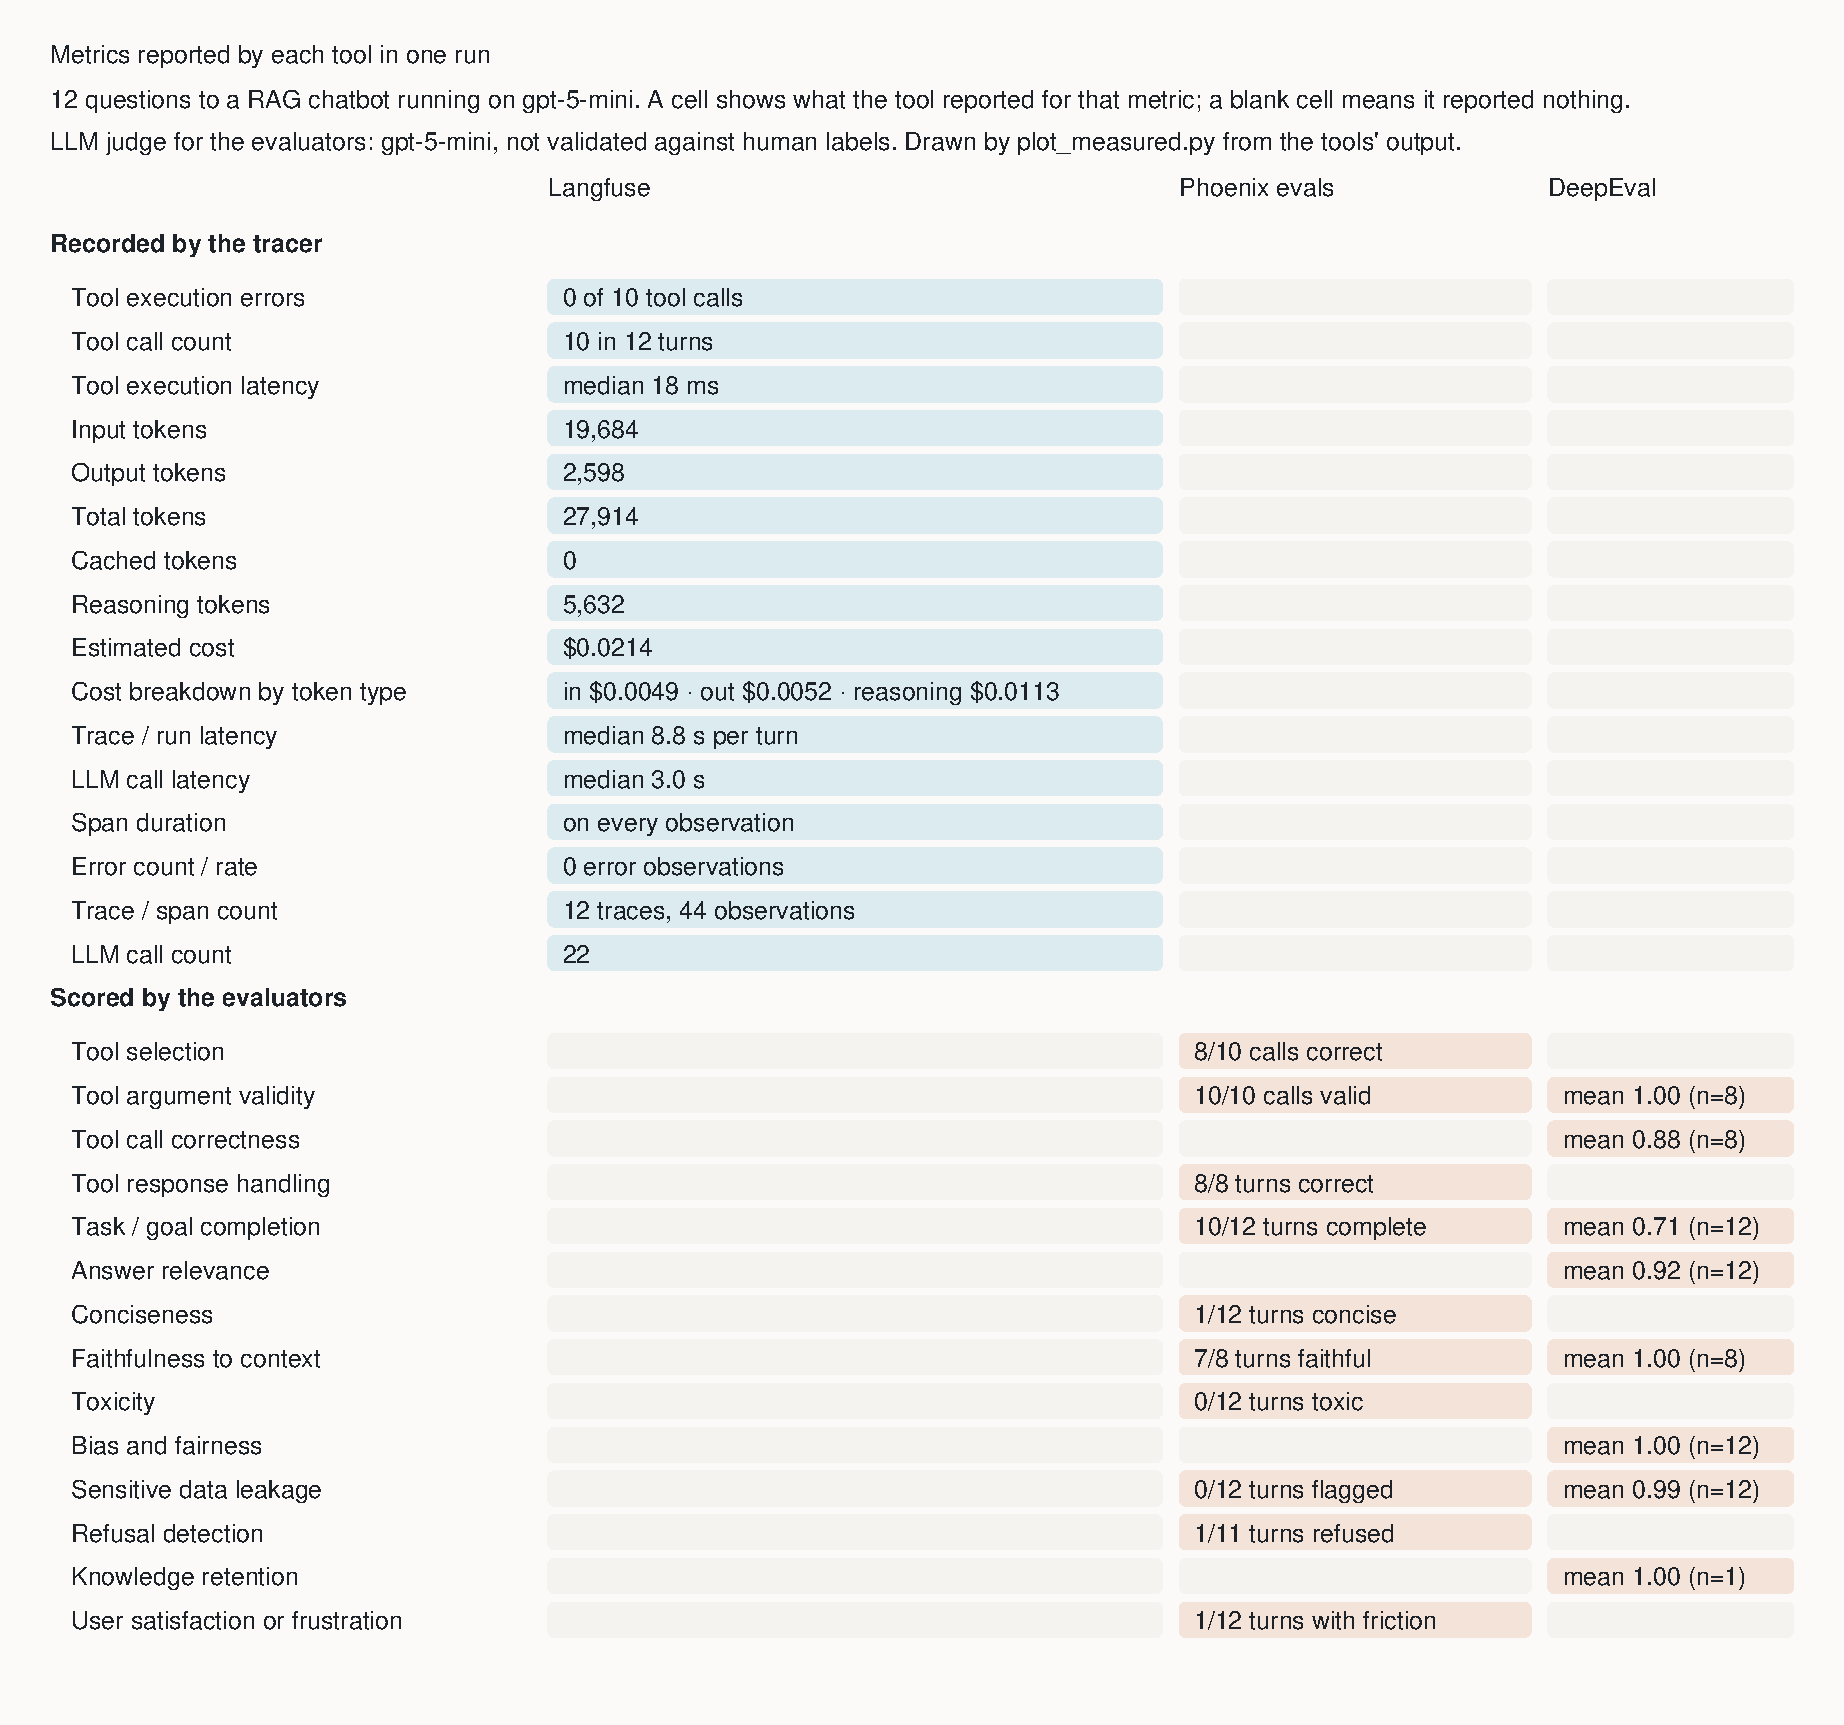
\includegraphics[width=0.78\textwidth]{figures/metrics_measured_20261028-104817.pdf}
\caption{Metrics reported by Langfuse (tracing) and by the Arize Phoenix and DeepEval evaluators for the 12-question run. Each row is a metric; a cell gives the measurement (tracer) or score (evaluators) the tool reported over the twelve runs. A blank means the tool reported nothing in this run, not that it lacks the metric: Langfuse was used only for tracing, and not every built-in evaluator was run. Drawn by the authors' script from the tools' output.}
\label{fig:example}
\end{figure*}

\subsubsection{Observations}
\begin{itemize}
  \item \textbf{Error metrics missed a failure the application did not flag.} In two of the twelve runs the course lookup failed (``No course found matching `MCP'\,''); the application returns this as an ordinary tool result, not as an error, so Langfuse's error counts stayed at zero although the message is in the recorded tool output: an error metric counts only what the application marks as an error. In one of them the second search recovered (Fig.~\ref{fig:graph}); in the other it led to a wrong answer, and DeepEval Task Completion scored 0.00, Phoenix Completeness said incomplete and DeepEval Tool Correctness scored 0.00.
  \item \textbf{Two tools disagreed on the same unique metric.} For the question the transcripts cannot answer, the answer said Kubernetes is not covered and then added Kubernetes instructions found nowhere in the retrieved text. Phoenix Faithfulness flagged it as unfaithful; DeepEval Faithfulness scored it 1.0. The two tool-specific metrics share a name and a property but not a procedure, which a unique metric does not show.
  \item \textbf{An off-target answer was visible.} When asked for an instructor's name, the application returned a lesson outline; DeepEval Answer Relevancy scored 0.30.
  \item \textbf{Conversation metrics behaved as expected on the one multi-turn conversation.} Knowledge Retention scored 1.0 because the application kept the user's earlier statement, and User Friction fired only on the turn in which the user complained. With one conversation, this shows that the metrics run, not that they are reliable.
\end{itemize}
DeepEval's Task Completion treats a plain question as a task to perform, so it can score a correct answer low (0.35 for ``What is the capital of Australia?''); its mean (0.71) should not be read as answer quality.

\section{Method}\label{sec:method}
This section describes how the 13 tools were found and selected, how their built-in metrics were collected from the documentation, and how those metrics were grouped into a taxonomy.

\begin{table*}[!t]
\centering
\footnotesize
\begin{tabular}{p{0.85in}p{1.7in}p{2.2in}p{1.6in}}
\toprule
Channel & Planned & Run & Result \\
\midrule
1. GitHub & 17 queries (10 topics, 7 keywords) on the REST API, 30 repositories each, at least 1,000 stars, not archived, pushed in the last six months & All 17 queries; 14 returned repositories & 182 distinct repositories; 37 kept (Table~\ref{tab:funnel}) \\
2. Google & 8 queries, first 30 results each, titles and snippets & 6 queries; the two ``comparison'' queries were planned but dropped; 173 results, 165 distinct URLs & 68 tools named; 13 kept \\
3. Standards & OpenTelemetry GenAI semantic conventions & Included as one entry & OpenTelemetry (a standard, not a product) \\
\bottomrule
\end{tabular}
\caption{The three search channels: plan and execution.}
\label{tab:channels}
\end{table*}

\subsection{Tool search}
The search adapts the multivocal approach of Garousi et al.~\cite{garousi2019guidelines}. Most tools are documented in repositories, vendor pages and blogs rather than in papers, so we search several kinds of source with fixed queries, apply written inclusion and exclusion rules, and log every query so the search can be repeated. The GitHub queries can be rerun through the API with the same limits; Google results depend on the date and the session, so that channel can be repeated but not reproduced exactly. We did not apply the whole guideline: sources were not graded for quality, and the search was not continued until no new tools appeared; each query has a fixed cut-off. The protocol has three channels; Table~\ref{tab:channels} shows what each was planned to do and what was run. All searches were run on 2026-10-22.

GitHub and Google find different things. GitHub returns only open-source repositories, and the star and activity limits (I2) are part of the query. Closed-source products have no repository, so they reach the study only through web search, and for them the corroboration rule I3 applies instead. Google returns both kinds, which is why eight tools appear in both channels. A closed-source tool that the first 30 results of the six queries do not name is absent (Section~\ref{sec:limits}).

\subsection{Inclusion, exclusion and selection}
The 42 candidate tools are not simply the two result lists with duplicates removed; they are what survives the written rules (Table~\ref{tab:funnel}). Each GitHub repository was checked by hand against I1 and E1--E4: 145 of the 182 were removed (68 unrelated, 57 tutorials or lists, 7 gateways, 7 agent-building frameworks, 6 model-level harnesses), leaving 37. The Google results were read for tool names, and each of the 68 tools named was screened with I1--I3, E1--E6 and the independent-source count, which kept 13; three benchmark candidates were removed as out of scope. The 42 candidates are the 37 GitHub tools plus the 5 tools only Google found; the 8 tools found by both count once (E5).

\begin{table}[!t]
\centering
\footnotesize
\begin{tabular}{llr}
\toprule
Stage & Rules & Count \\
\midrule
GitHub: repositories returned & I2 (in query) & 182 \\
\quad kept after manual check & I1, E1--E4 & 37 \\
Google: tools named & -- & 68 \\
\quad kept & I1--I3, E1--E6, C1 & 13 \\
Candidates (merged) & E5 & 42 \\
Scope screening & S1 & 31 \\
Relevance, corroboration & A1, C1 & 13 \\
\bottomrule
\end{tabular}
\caption{From search results to the 13 selected tools.}
\label{tab:funnel}
\end{table}

A tool is included if its primary purpose is tracing, monitoring or evaluating LLM applications or agents (I1). Open-source tools need at least 1,000 stars, must not be archived and need a push or release in the last six months (I2). Closed-source tools need public documentation and mentions in at least two independent sources (I3). We exclude gateways and proxies, agent-building frameworks, model-level benchmark harnesses, tutorials and lists, and duplicates (E1--E5).
Three rules were added after the first Google run, and we report them as amendments to the protocol:
\begin{itemize}
  \item \textbf{E6}: general-purpose observability, APM, data, security or ML platforms whose LLM support is only a module are excluded, unless the LLM product is distributed on its own (for example Weights \& Biases Weave).
  \item \textbf{A1} (agent relevance): the tool's official documentation must explicitly cover agents, tool calls or multi-step traces. For each tool the evidence is a quote checked against a saved copy of the page.
  \item \textbf{C1} (corroboration): a tool enters the study only if at least two independent sources name it; the tool's own website does not count.
\end{itemize}
The scope screening (S1) keeps a tool whose own description gives observability or evaluation of LLM applications or agents as its primary purpose; it kept 31 of the 42 candidates and removed 10, with one borderline case treated as out. Each kept tool received one role (S2): \emph{standard} (telemetry conventions or instrumentation libraries), \emph{platform} (an application that stores and shows traces and offers evaluation or monitoring) or \emph{framework} (a library or CLI that runs evaluations, with no trace backend of its own). After A1 and C1, 13 tools remained; the other 18 S1 tools had no independent source, because a tool found only on GitHub has no Google source to count. C1 applies to open-source tools as well, which is stricter than the inclusion rule I3 (two sources for closed-source tools only); in effect, Google corroboration decides the final set, and GitHub supplies candidates that Google also names (MLflow and Evidently passed I2 but were removed by C1). The 13 are ranked by the number of independent Google sources, then by GitHub stars. The ranking rule was fixed before metric coverage and download counts were examined, and download counts are reported only as corroboration.

\subsection{Collecting built-in metrics}
For each selected tool we read its official documentation and recorded every \emph{built-in} metric: one the tool itself ships, as opposed to a user-written or user-defined metric, a community or third-party metric, or one available only through an integration. Each row stores the documentation URL, a verbatim quote, the saved plain-text copy of the page and the access date, and a script checks that every quote appears word for word in its saved page.
A scope rule (M1) keeps only metrics that describe how an agent run executes (tool use, task and goal, plan and trajectory, tokens, cost, latency, errors and counts) or how good its output is (answer quality, grounding, safety and conversation). Text-match and format checks, retrieval scores, audio, voice and image metrics, task-specific output metrics and custom judges are out of scope. A metric that restates one already in the taxonomy is merged into it, not added; a metric provided by a single tool is kept. M1 removed 252 rows and kept 241, so the taxonomy covers about half of what the tools document; the removed rows, with the reason for each, are kept with the data.

\subsection{Building the taxonomy}\label{sec:taxonomy}
Two tool-specific metrics are merged into one unique metric when they measure the same property, whatever the tools call them. The object is usually the same (a tool call, an agent run, an LLM call or a token type); where tools compute the property on different objects, as for task completion on a response, a run or a conversation, the definition says so. Merging is by property, not by procedure: the tool-specific metrics in one unique metric may compute it differently. The mapping from tool-specific names to unique metrics (274 pairs) is made by hand and kept with the data; the definitions of the unique metrics are written by the authors and are not quoted from the documentation. A metric is typed as \emph{Observability} if its values are captured from a run or derived from what was captured, and as \emph{Evaluation} if its values are scores, that is, judgements of agent behaviour or output (Section~\ref{sec:terms}).
For each tool and metric the matrix records the strongest status found: built-in, integration, community, template, generic custom, records scores or not documented. The last status means nothing was found in the pages read, which is not proof that the tool lacks the capability.

\FloatBarrier
\section{Results}\label{sec:results}
This section presents the 13 selected tools, then the built-in metrics they document and the taxonomy that groups them.

\subsection{The 13 selected tools}
\begin{table*}[!t]
\centering
\small
\begin{tabular}{rlllrrl}
\toprule
\# & Tool & Role & Found via & Stars & Indep.\ sources & OTel link \\
\midrule
1 & Arize Phoenix~\cite{tool_arize_phoenix} & platform & GitHub + Google & 11{,}951 & 16 & built on \\
2 & Langfuse~\cite{tool_langfuse} & platform & GitHub + Google & 36{,}193 & 15 & built on \\
3 & LangSmith~\cite{tool_langsmith} & platform & Google only & -- & 13 & accepts \\
4 & DeepEval~\cite{tool_deepeval} & framework & GitHub + Google & 19{,}039 & 12 & not found \\
5 & OpenTelemetry~\cite{tool_opentelemetry} & standard & Google only & -- & 10 & defines \\
6 & Helicone~\cite{tool_helicone} & platform & GitHub + Google & 6{,}232 & 6 & not found \\
7 & Braintrust~\cite{tool_braintrust} & platform & Google only & -- & 5 & accepts \\
8 & promptfoo~\cite{tool_promptfoo} & framework & GitHub + Google & 26{,}286 & 4 & optional \\
9 & OpenLLMetry~\cite{tool_openllmetry} & standard & GitHub + Google & 7{,}501 & 4 & built on \\
10 & Opik~\cite{tool_opik} & platform & GitHub + Google & 22{,}833 & 3 & accepts \\
11 & Galileo~\cite{tool_galileo} & platform & Google only & -- & 3 & accepts \\
12 & OpenInference~\cite{tool_openinference} & standard & GitHub + Google & 1{,}278 & 2 & built on \\
13 & Weights \& Biases Weave~\cite{tool_weights_biases_weave} & platform & Google only & -- & 2 & span-like \\
\bottomrule
\end{tabular}
\caption{The 13 selected tools, ranked by independent Google sources (``Indep.\ sources''), then GitHub stars. Stars were read on 2026-10-22 and are blank for tools without a GitHub result. ``OTel link'' is how the tool's documentation relates it to OpenTelemetry: it defines the conventions, is built on OpenTelemetry, accepts OpenTelemetry traces, offers optional OpenTelemetry tracing, or models its data like spans; ``not found'' means nothing was found in the pages read (evidence in \texttt{tool\_relations.csv}).}
\label{tab:tools}
\end{table*}

Table~\ref{tab:tools} lists the 13 tools in rank order with their role, GitHub stars where the tool is open source, and the number of independent Google sources. Five tools were found through Google only. Each tool has one role, which says what kind of thing it is:
\begin{itemize}
  \item \textbf{Platform} (8 tools: Phoenix, Langfuse, LangSmith, Helicone, Braintrust, Opik, Galileo, Weave). An application, hosted or self-hosted, that stores and shows traces of agent runs and also offers evaluation or monitoring on top of them. This is what most people mean by an observability tool: an SDK sends the data in, and the platform stores it, draws dashboards and scores runs.
  \item \textbf{Framework} (2 tools: DeepEval, promptfoo). A library or command-line program that runs evaluations or tests on an application's outputs. It has no trace storage or interface of its own; its metrics are computed when the user runs it, and the results are read in the terminal, in files or in a separate service.
  \item \textbf{Standard} (3 tools: OpenTelemetry, OpenLLMetry, OpenInference). A shared vocabulary for telemetry, or an instrumentation library that emits it: OpenTelemetry defines the conventions, and OpenInference and OpenLLMetry attach them to LLM and agent libraries. They have no backend or evaluators; they define what a trace contains, so the metrics they list are names of attributes that other tools read. \todo{Fig.~\ref{fig:taxonomy} credits OpenLLMetry with 13 evaluation metrics, against none for the other two standards. Check whether these are Traceloop platform evaluators documented alongside OpenLLMetry; if so, say why they count, or move them.}
\end{itemize}
The role is a single label chosen from each tool's own description, so a tool that also ships a smaller component of another kind (Phoenix, for example, has an evaluation library) is labelled by its main purpose. The roles matter when reading the metric tables: a platform computes and shows a metric, a framework computes it when run, and a standard only names it. \todo{Comment on the mix of roles and of open and closed source once final.}

\subsection{Built-in metrics and taxonomy}
The 13 tools document 241 built-in metrics that pass the scope rule, which map to 46 unique metrics in 13 categories (Fig.~\ref{fig:taxonomy}); the 13 categories use 11 names, two of which appear under both types. Nineteen are Observability metrics and 27 are Evaluation metrics.

% Empty float: without it LaTeX leaves the left column of the Discussion page empty (two-column float-page quirk).
\begin{table}[t]
\mbox{}
\end{table}

\begin{figure*}[!t]
\centering
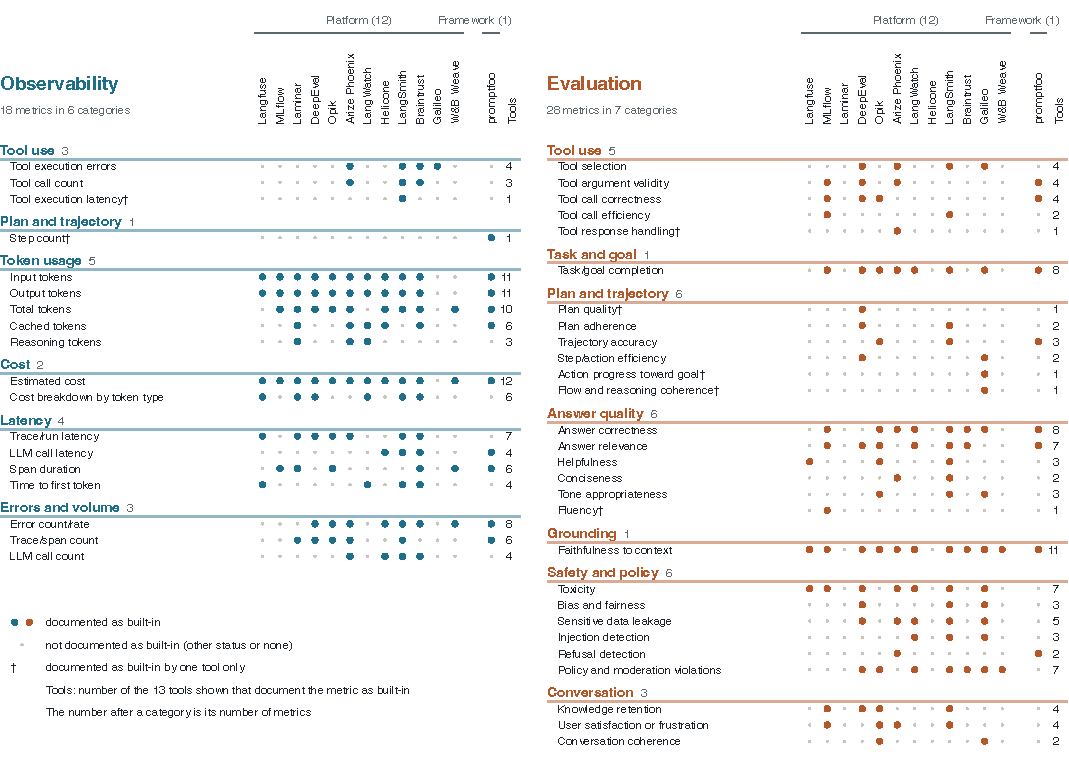
\includegraphics[width=\textwidth]{figures/metric_taxonomy_coverage.pdf}
\caption{The metric taxonomy and the tools that document each metric as built-in. Rows are the 46 unique metrics, grouped by type and category; columns are the 13 tools, grouped by role and in the order of Table~\ref{tab:tools} within each role. A coloured dot means the tool documents the metric as built-in; a grey dot means another status or nothing found (Section~\ref{sec:taxonomy}); a dagger marks a metric that only one tool documents as built-in. Definitions are in Table~\ref{tab:defs}.}
\label{fig:taxonomy}
\end{figure*}

Coverage is uneven. 17 of the 46 metrics are documented as built-in by at least five of the 13 tools, and 3 of them (input tokens, output tokens, faithfulness to context) by ten; 5 metrics are provided by exactly one tool (Step count, tool call efficiency, tool response handling, plan quality, action progress toward goal).
These counts include the three standards, which name attributes rather than compute metrics; they supply 25 of the 102 built-in observability cells and 13 of the 99 evaluation cells. Counting only the ten platforms and frameworks, 12 metrics reach five tools, faithfulness to context (9 tools) and estimated cost (8) are the most widely documented, and time per output token is documented by standards only.
Fig.~\ref{fig:taxonomy} shows the taxonomy together with the tools that document each metric as built-in, and Table~\ref{tab:defs} defines each metric.

\begin{table*}[t]
\centering
\scriptsize
\setlength{\tabcolsep}{4pt}
\begin{tabular}{@{}p{1.95in}p{5.0in}@{}}
\toprule
Metric & Definition \\
\midrule
\multicolumn{2}{@{}l}{\textbf{Observability} (19 metrics)} \\
\addlinespace[1.5pt]
\multicolumn{2}{@{}l}{\textit{Tool use}} \\
\quad Tool execution errors & Count, rate or detection of failed tool executions. \\
\quad Tool call count & Number of tool calls made by an agent run. \\
\quad Tool execution latency & Time taken by tool executions. \\
\addlinespace[1.5pt]
\multicolumn{2}{@{}l}{\textit{Plan and trajectory}} \\
\quad Step count$^\dagger$ & Number of steps in an agent run. \\
\addlinespace[1.5pt]
\multicolumn{2}{@{}l}{\textit{Token usage}} \\
\quad Input tokens & Number of tokens sent to the model (prompt). \\
\quad Output tokens & Number of tokens generated by the model (completion). \\
\quad Total tokens & Total number of tokens for a call, trace or model: input plus output, plus reasoning tokens where a tool counts them separately. \\
\quad Cached tokens & Input tokens read from or written to a provider-side cache. \\
\quad Reasoning tokens & Tokens spent on model reasoning; some tools count them within output tokens, others separately. \\
\addlinespace[1.5pt]
\multicolumn{2}{@{}l}{\textit{Cost}} \\
\quad Estimated cost & Monetary cost of model usage, computed from token counts and model prices. \\
\quad Cost breakdown by token type & Cost split by input, output, cached or other token type. \\
\addlinespace[1.5pt]
\multicolumn{2}{@{}l}{\textit{Latency}} \\
\quad Trace/run latency & End-to-end duration of an agent run, workflow or trace. \\
\quad LLM call latency & Duration of a single model call. \\
\quad Span duration & Duration of an individual span or step of a trace (generic, not specific to LLM or tool spans). \\
\quad Time to first token & Time from request to the first generated token. \\
\quad Time per output token/generation time & Time spent generating tokens after the first one. \\
\addlinespace[1.5pt]
\multicolumn{2}{@{}l}{\textit{Errors and volume}} \\
\quad Error count/rate & Count or rate of failed runs, traces, spans or model calls. \\
\quad Trace/span count & Number of traces or spans recorded. \\
\quad LLM call count & Number of model (inference) calls. \\
\midrule
\multicolumn{2}{@{}l}{\textbf{Evaluation} (27 metrics)} \\
\addlinespace[1.5pt]
\multicolumn{2}{@{}l}{\textit{Tool use}} \\
\quad Tool selection & Whether the agent chose the appropriate tool for the task. \\
\quad Tool argument validity & Whether the arguments of a tool call are correct and well-formed (for example against the tool's schema or expected values). \\
\quad Tool call correctness & Whether the tool calls the agent made match the calls expected or appropriate for the task. \\
\quad Tool call efficiency$^\dagger$ & Whether the agent called tools without redundant or unnecessary calls. \\
\quad Tool response handling$^\dagger$ & Whether the agent correctly processed what a tool returned, including errors. \\
\addlinespace[1.5pt]
\multicolumn{2}{@{}l}{\textit{Task and goal}} \\
\quad Task/goal completion & Whether the agent completed the task or achieved the goal it was given, judged on a run, a conversation or a response. \\
\addlinespace[1.5pt]
\multicolumn{2}{@{}l}{\textit{Plan and trajectory}} \\
\quad Plan quality$^\dagger$ & Quality of the plan the agent produced. \\
\quad Plan adherence & Whether the agent's actions followed its own plan. \\
\quad Trajectory accuracy & Whether the sequence of agent steps and tool calls was logical or matches a reference trajectory. \\
\quad Step/action efficiency & Whether the agent reached the goal with a minimal number of steps. \\
\quad Action progress toward goal$^\dagger$ & Whether each action moved the agent closer to its goal. \\
\quad Flow and reasoning coherence & Whether the agent's sequence of actions and reasoning steps is logically consistent. \\
\addlinespace[1.5pt]
\multicolumn{2}{@{}l}{\textit{Answer quality}} \\
\quad Answer correctness & Whether the agent's answer is factually correct, judged by a model or against a reference answer. \\
\quad Answer relevance & Whether a response addresses the user's input, per answer or per turn, without off-topic content. \\
\quad Helpfulness & How useful or helpful the answer is to the user. \\
\quad Conciseness & Whether the answer gives the requested information without unnecessary or padded content. \\
\quad Tone appropriateness & Whether the tone of the response is appropriate for the context. \\
\addlinespace[1.5pt]
\multicolumn{2}{@{}l}{\textit{Grounding}} \\
\quad Faithfulness to context & Whether the claims in the answer are supported by the provided context. Unsupported or contradicted claims count as hallucination. \\
\addlinespace[1.5pt]
\multicolumn{2}{@{}l}{\textit{Safety and policy}} \\
\quad Toxicity & Whether the output contains toxic, abusive, hateful or profane language. \\
\quad Bias and fairness & Whether the output contains bias, stereotyping or discrimination against a person or group. \\
\quad Sensitive data leakage & Whether the input or output exposes personal data or secrets (for example PII, credentials). \\
\quad Injection detection & Whether an input contains an injection attempt (prompt, code or SQL injection) aimed at the agent. \\
\quad Refusal detection & Whether the model refuses, declines or avoids answering a request. \\
\quad Policy and moderation violations & Whether the output breaks a safety, moderation, compliance or content policy. \\
\addlinespace[1.5pt]
\multicolumn{2}{@{}l}{\textit{Conversation}} \\
\quad Knowledge retention & Whether the agent remembers and uses facts the user gave earlier in the conversation. \\
\quad User satisfaction or frustration & Whether the user's messages show satisfaction, or frustration, corrections and repeated attempts. \\
\quad Conversation coherence & Coherence and quality of the messages in a conversation, including repetition or degeneration. It scores the dialogue, not the agent's sequence of actions. \\
\bottomrule
\end{tabular}

\caption{Definitions of the 46 unique metrics, in the authors' wording, grouped as in Fig.~\ref{fig:taxonomy}, which shows the tools that document each metric as built-in. A dagger marks a metric that only one tool documents as built-in.}
\label{tab:defs}
\end{table*}

\todo{Add the tool-by-metric matrix as a figure (export \texttt{results/tool\_metric\_matrix.html} to PDF) and describe the status counts: of the 598 cells, 201 are built-in, 168 generic custom, 81 records scores, 145 not documented, 2 integration and 1 template.}

\FloatBarrier
\section{Discussion}\label{sec:discussion}
\todo{Interpret: the split between measurements and judgements; metrics most tools share (token usage, cost, faithfulness) versus metrics only one tool offers (step count, tool call efficiency, tool response handling, plan quality, action progress toward goal); why the same metric name can mean different things in different tools; what the example suggests about combining tracing with evaluators; which metrics no tool reported in the example (plan, trajectory, step, helpfulness, tone, injection, policy, conversation coherence).}

\section{Limitations}\label{sec:limits}
\begin{itemize}
  \item \textbf{Search strategy.} We could not include every tool, so the search follows fixed rules. Selection by corroboration (C1) reduced the list to 13 tools; widely used tools with no third-party mention in the first 30 results of the six Google queries are absent, and the counts reflect what ranks in those queries, not usage. Google counts come from titles and snippets only, only six of the eight planned queries were run, and the region and language of the search session were not recorded (the searches ran in a private browser window). Cloud-vendor products that appear only under vendor-site queries were not searched for. A source counts as independent if it is not the tool's own website, so a competitor's comparison post counts; the source counts measure visibility, not independent assessment. Ranking by stars favours open-source tools.
  \item \textbf{Scope.} Benchmarks and evaluation harnesses are out of scope, so metrics such as pass$^k$ that come from them are not in the tables. The metric scope rule M1 removed about half of the documented rows, including retrieval scores, which many RAG applications rely on.
  \item \textbf{Documentation only.} Metrics come from official documentation pages. A metric present only in source code is not listed, and a cell marked ``not documented'' is not proof of absence. Row counts are not comparable across tools, because some documentation lists individual assertion types and other lists fewer, broader metrics.
  \item \textbf{Shared foundations.} Several tools build on the same conventions (Section~\ref{sec:stack}), so two tools documenting the same observability metric are not independent designs, and the number of tools per metric measures documentation overlap, not independent adoption. Section~\ref{sec:results} therefore also gives the counts without the three standards.
  \item \textbf{Taxonomy.} The mapping of tool-specific metrics to unique metrics and the metric definitions are the authors' judgement. A finer or coarser split of properties would change the count of 46. \todo{State any validation, such as a second coder.}
  \item \textbf{Example.} One run of twelve questions on one application, with one small model acting as both application and judge and no human labels. Evaluator scores illustrate what each tool reports; they do not measure the accuracy of the tools. The example uses three of the 13 tools.
\end{itemize}

\section{Conclusion}
\todo{Summarise the contributions and the main finding; state future work (for example validating evaluator scores against human labels, extending the example to a multi-agent application).}

\section*{Data availability}
\todo{Repository URL and archive (for example Zenodo). The repository holds the search logs, the evidence tables with quotes and saved pages, the taxonomy and mapping, and the example's scripts and results. The example's course transcripts are not redistributed.}

\bibliographystyle{IEEEtran}
\bibliography{references}

\end{document}
